% The `linenumber` option is necessary for ease of reviewer referencing



\documentclass[linenumber]{jdsart}

\volume{0}
\issue{0}
\pubyear{2025}
\articletype{research-article}
\doi{0000}

%startlocaldefs
%% Put your local definitions here

% local macros
%\newtheorem{thm}{Theorem}
%\newtheorem{prop}{Proposition}
%\newtheorem{cor}{Corollary}
%\newtheorem{lem}{Lemma}

%\theoremstyle{remark}
%\newtheorem{defn}{Definition}
%\newtheorem{rem}{Remark}
%\newtheorem{exmp}{Example}
%\newtheorem{note}{Note}

%endlocaldefs
\usepackage{tikz}
\usetikzlibrary{arrows.meta,calc}
\usepackage{xcolor}
\usepackage{graphicx}
\usepackage{placeins}

\definecolor{figbg}{RGB}{245,247,251}
\definecolor{figdark}{RGB}{39,49,66}
\definecolor{figmid}{RGB}{95,111,141}
\definecolor{figblue}{RGB}{31,119,180}
\definecolor{figedge}{RGB}{53,92,125}
\definecolor{figlight}{RGB}{199,209,223}

\begin{document}



\begin{frontmatter}

\title{A Statistical Workflow for Interpretable Reduced-Form Surrogates from Large Simulators: A Case Study with the Bioenergy Scenario Model}
\runtitle{Reduced-Form Surrogates for Large Simulators}
%\title{\thanksref{t1}}
%\thankstext[id=t1]{}

\author[1]{\inits{D.}\fnms{Dylan}~\snm{Hettinger}\thanksref{t1}\ead{dylan.hettinger@nlr.gov}}
\author[2]{\inits{S.}\fnms{Steve}~\snm{Peterson}\ead{steve@evans-peterson.com}}
\author[1]{\inits{C.}\fnms{Colby}~\snm{Smith}\ead{colby.smith@nlr.gov}}
\author[1]{\inits{E.}\fnms{Emily}~\snm{Newes}\ead{emily.newes@nlr.gov}}

\thankstext[type=corresp,id=t1]{Corresponding author.}

\address[1]{\institution{National Laboratory of the Rockies (NLR)}, \cny{Golden, Colorado, USA}}
\address[2]{\institution{[Steve Peterson affiliation]}, \cny{[City, State, USA]}}

%\runtitle{}  %use if necessary to change auto-generated
%\runauthor{} %use if necessary to change auto-generated

%\dedicated{}

\begin{abstract} % avoid notations; avoid citations; no exceeding 250 words
Large simulators can generate input--output problems whose dimensionality makes direct reduced-form modeling, classical global sensitivity analysis, and integration into downstream studies operationally difficult. We present a staged statistical workflow for converting such problems into interpretable reduced-form surrogates by combining regression screening against permutation null distributions, SHapley Additive exPlanations (SHAP)-based interaction discovery, generalized additive model--based nonlinear transformation discovery, penalized regression, and final unpenalized ordinary least squares estimation. We demonstrate the workflow on the Bioenergy Scenario Model, a large-scale system dynamics model of U.S. biofuels deployment. In this case study, 160 exogenous inputs and 635 time-series outputs were mapped to 23,495 scalar responses for modeling. Performance was evaluated on a 10\% holdout sample excluded from every stage of screening, selection, and estimation. The final ordinary least squares reduced form achieved an nRMSE of 0.0445 using 340 retained predictors derived from 62 first-order inputs. The resulting reduced form preserves interpretability and yields a portable surrogate for downstream analysis without rerunning the full simulator and demonstrates the efficacy of the statistical workflow.
\end{abstract}

\begin{keywords} % Alphabetical; not to repeat anything in the title
\kwd{interpretable surrogate}
\kwd{reduced-form model}
\kwd{simulator workflow}
\end{keywords}

\end{frontmatter}

\section{Introduction}
\label{sec:introduction}

Large simulators now create a class of statistical problems in which the challenge is not merely prediction from expensive runs, but compression of a high-dimensional input--output map into a reduced form that is computationally cheap, portable, and interpretable enough for downstream scientific and policy analysis. In this setting, the central task is to move from a large-data simulator regime \citep{Donoho2017} to a statistically manageable high-dimensional reduced-form regime \citep{Wainwright2019} without losing the main structure needed for explanation, prediction, and subsequent use \citep{Shmueli2010}.

The main statistical foundation for this problem comes from the design and analysis of computer experiments \citep{SacksEtAl1989,SantnerWilliamsNotz2018} and from surrogate modeling for complex simulators \citep{Gramacy2020}. Within that literature, surrogate models are used for prediction, uncertainty quantification, and calibration \citep{KennedyOHagan2001,Gramacy2020}. When simulators produce many outputs, basis representations and related output-reduction strategies are often introduced before emulation or calibration \citep{HigdonEtAl2008}. A separate line of work in statistics and interpretable machine learning emphasizes additive representations \citep{HastieTibshirani1990}, sparse linear models \citep{Tibshirani1996}, hierarchical interaction structures \citep{BienTaylorTibshirani2013}, and model classes whose structure can be communicated directly rather than explained post hoc \citep{Rudin2019,AllenGanZheng2024}. The workflow proposed here sits at the intersection of these traditions: it uses calibrated screening, structured feature discovery, and sparse reduction to compress a large simulator problem into a smaller statistical problem, but it deliberately ends in an interpretable algebraic reduced form rather than a black-box emulator.

Two scaling pressures make this reduction problem difficult. On the input side, even moderate numbers of exogenous drivers can generate very large candidate libraries once interactions and simple nonlinear transformations are introduced. On the output side, large simulators often return many correlated quantities across time, space, or scenario dimensions, so the analyst must reduce not only predictor complexity but also output multiplicity. Downstream tasks such as scenario exploration, uncertainty analysis, sensitivity analysis, and coupling to other models are therefore often limited not by the simulator itself, but by the absence of a compact external representation that can be evaluated, inspected, and communicated outside the original software environment.

This paper presents a workflow for constructing interpretable reduced-form surrogates in such settings. The workflow separates the problem into distinct stages: defining an external input--output interface, expanding an algebraic candidate feature space, conditioning outputs for discovery, screening against a calibrated null, stabilizing sparse support selection, and fitting a final unpenalized ordinary least squares representation. A holdout split is reserved before any adaptive modeling step and is used only for final validation.

The contribution is therefore methodological in design. First, we formulate the surrogate task as a big-to-small statistical reduction problem in which both input-space and output-space growth must be controlled. Second, we present a staged workflow that links interface definition, screening, discovery, selection, estimation, prediction, validation, and interpretation into a coherent pipeline aimed at interpretability, tractability, and reproducibility. Third, we demonstrate in a demanding case study that this workflow can yield a high-fidelity reduced form while preserving portability and algebraic transparency. The remainder of the paper formalizes the generic problem, details the workflow, presents the case study and results, and then discusses scope, limitations, conclusions, and reproducibility.

\section{Problem Formulation}
\label{sec:problem}

For simulator run $i=1,\dots,n$, let
\[
x_i \in \mathbb{R}^d
\]
denote the vector of exogenous inputs.
%The components of $x_i$ may represent continuous variables, integer-valued settings, or binary indicators coded numerically as needed; at this level of abstraction, they are treated uniformly as externally szpecified drivers rather than simulator-internal states.
Stacking the model runs gives the input matrix
\[
U =
\begin{bmatrix}
x_1^{\top} \\
\vdots \\
x_n^{\top}
\end{bmatrix}
\in \mathbb{R}^{n \times d}.
\]
% The key modeling restriction is not the input type, but the interface: the reduced form should depend only on exogenous quantities that can be sampled, documented, and reused outside the full simulator.

To extend the feature space, we then construct an algebraic feature library
\[
\phi(x_i) \in \mathbb{R}^k
\]
whose coordinates include first-order terms, selected pairwise interactions, and selected simple nonlinear transformations of individual inputs. In the simplest form, this means starting with the original inputs, then augmenting them with terms such as $x_jx_\ell$ and $g(x_j)$ for a set of transformations $g$. The same construction can be extended to third-order or higher-order interactions if there is scientific or empirical reason to believe that such structure is necessary. Stacking the transformed runs yields the design matrix
\[
X =
\begin{bmatrix}
\phi(x_1)^{\top} \\
\vdots \\
\phi(x_n)^{\top}
\end{bmatrix}
\in \mathbb{R}^{n \times k}.
\]
Here, $U$ defines the scientific input space, while $X$ defines the statistical representation used to approximate the simulator with an interpretable algebraic surrogate.

Let
\[
y_i \in \mathbb{R}^p
\]
denote the vector of outputs for run $i$, and let
\[
Y =
\begin{bmatrix}
y_1^{\top} \\
\vdots \\
y_n^{\top}
\end{bmatrix}
\in \mathbb{R}^{n \times p}.
\]
The dimension $p$ may be large because outputs are often stacked across variables and over indexing dimensions such as time or space. This representation is standard when simulator responses are naturally functional or otherwise high-dimensional. For example, in the sensitivity-analysis literature, model outputs indexed over a continuum have been treated explicitly as functions \citep{CampbellMcKayWilliams2006}, dynamic simulator responses have been analyzed as multivariate outputs \citep{LamboniMonodMakowski2011}, and Sobol-type sensitivity analysis has been generalized to multidimensional and functional outputs \citep{GamboaJanonKleinLagnoux2014}. On the emulation and calibration side, high-dimensional simulator outputs are also commonly reduced through basis representations before statistical modeling \citep{HigdonGattikerWilliamsRightley2008}.

When $p$ is too large for some intermediate discovery steps, we allow a temporary reduced-response representation based on standardized outputs. Let $\widetilde{Y}$ denote the column-standardized version of $Y$, and define
\[
Z = \mathcal{R}(\widetilde{Y}) \in \mathbb{R}^{n \times r},
\qquad r \ll p,
\]
where $\mathcal{R}$ is a deterministic output-reduction operator. In this paper, $\mathcal{R}$ may be taken generically to mean projection onto a low-dimensional basis, such as the first $r$ principal component directions,
\[
\mathcal{R}(\widetilde{Y}) = \widetilde{Y}W_r,
\qquad
W_r \in \mathbb{R}^{p \times r},
\qquad
W_r^{\top}W_r = I_r.
\]
This reduced representation is used only as a computational device for screening and discovery. The final reduced form is always estimated and reported on the original response matrix $Y$, not on the reduced scores.

Because inputs can vary widely in numerical range, columns of $X$ are standardized before coefficient comparison and penalized fitting so that shrinkage and effect magnitudes are not driven by units alone \citep{HastieTibshiraniFriedman2009}. When output reduction is used, it is applied to standardized outputs for the analogous reason: high-variance responses should not dominate the retained directions of variation merely because of scale \citep{Jolliffe2002}.

The object of interest is therefore a sparse index set
\[
S \subset \{1,\dots,k\}
\]
and a coefficient matrix
\[
B_S \in \mathbb{R}^{|S| \times p}
\]
such that
\[
\widehat{Y} = X_S B_S
\]
predicts $Y$ well on held-out runs. Equivalently, once $S$ has been selected, the final reduced form is a multivariate linear model on a chosen algebraic basis. The statistical problem is therefore not only coefficient estimation. It is the joint problem of constructing a feature library rich enough to capture important structure, reducing that library to a stable and portable support, and retaining only terms that keep the final artifact interpretable, auditable, and reusable.

\begin{figure}[p]
\centering
\resizebox{0.94\linewidth}{!}{%
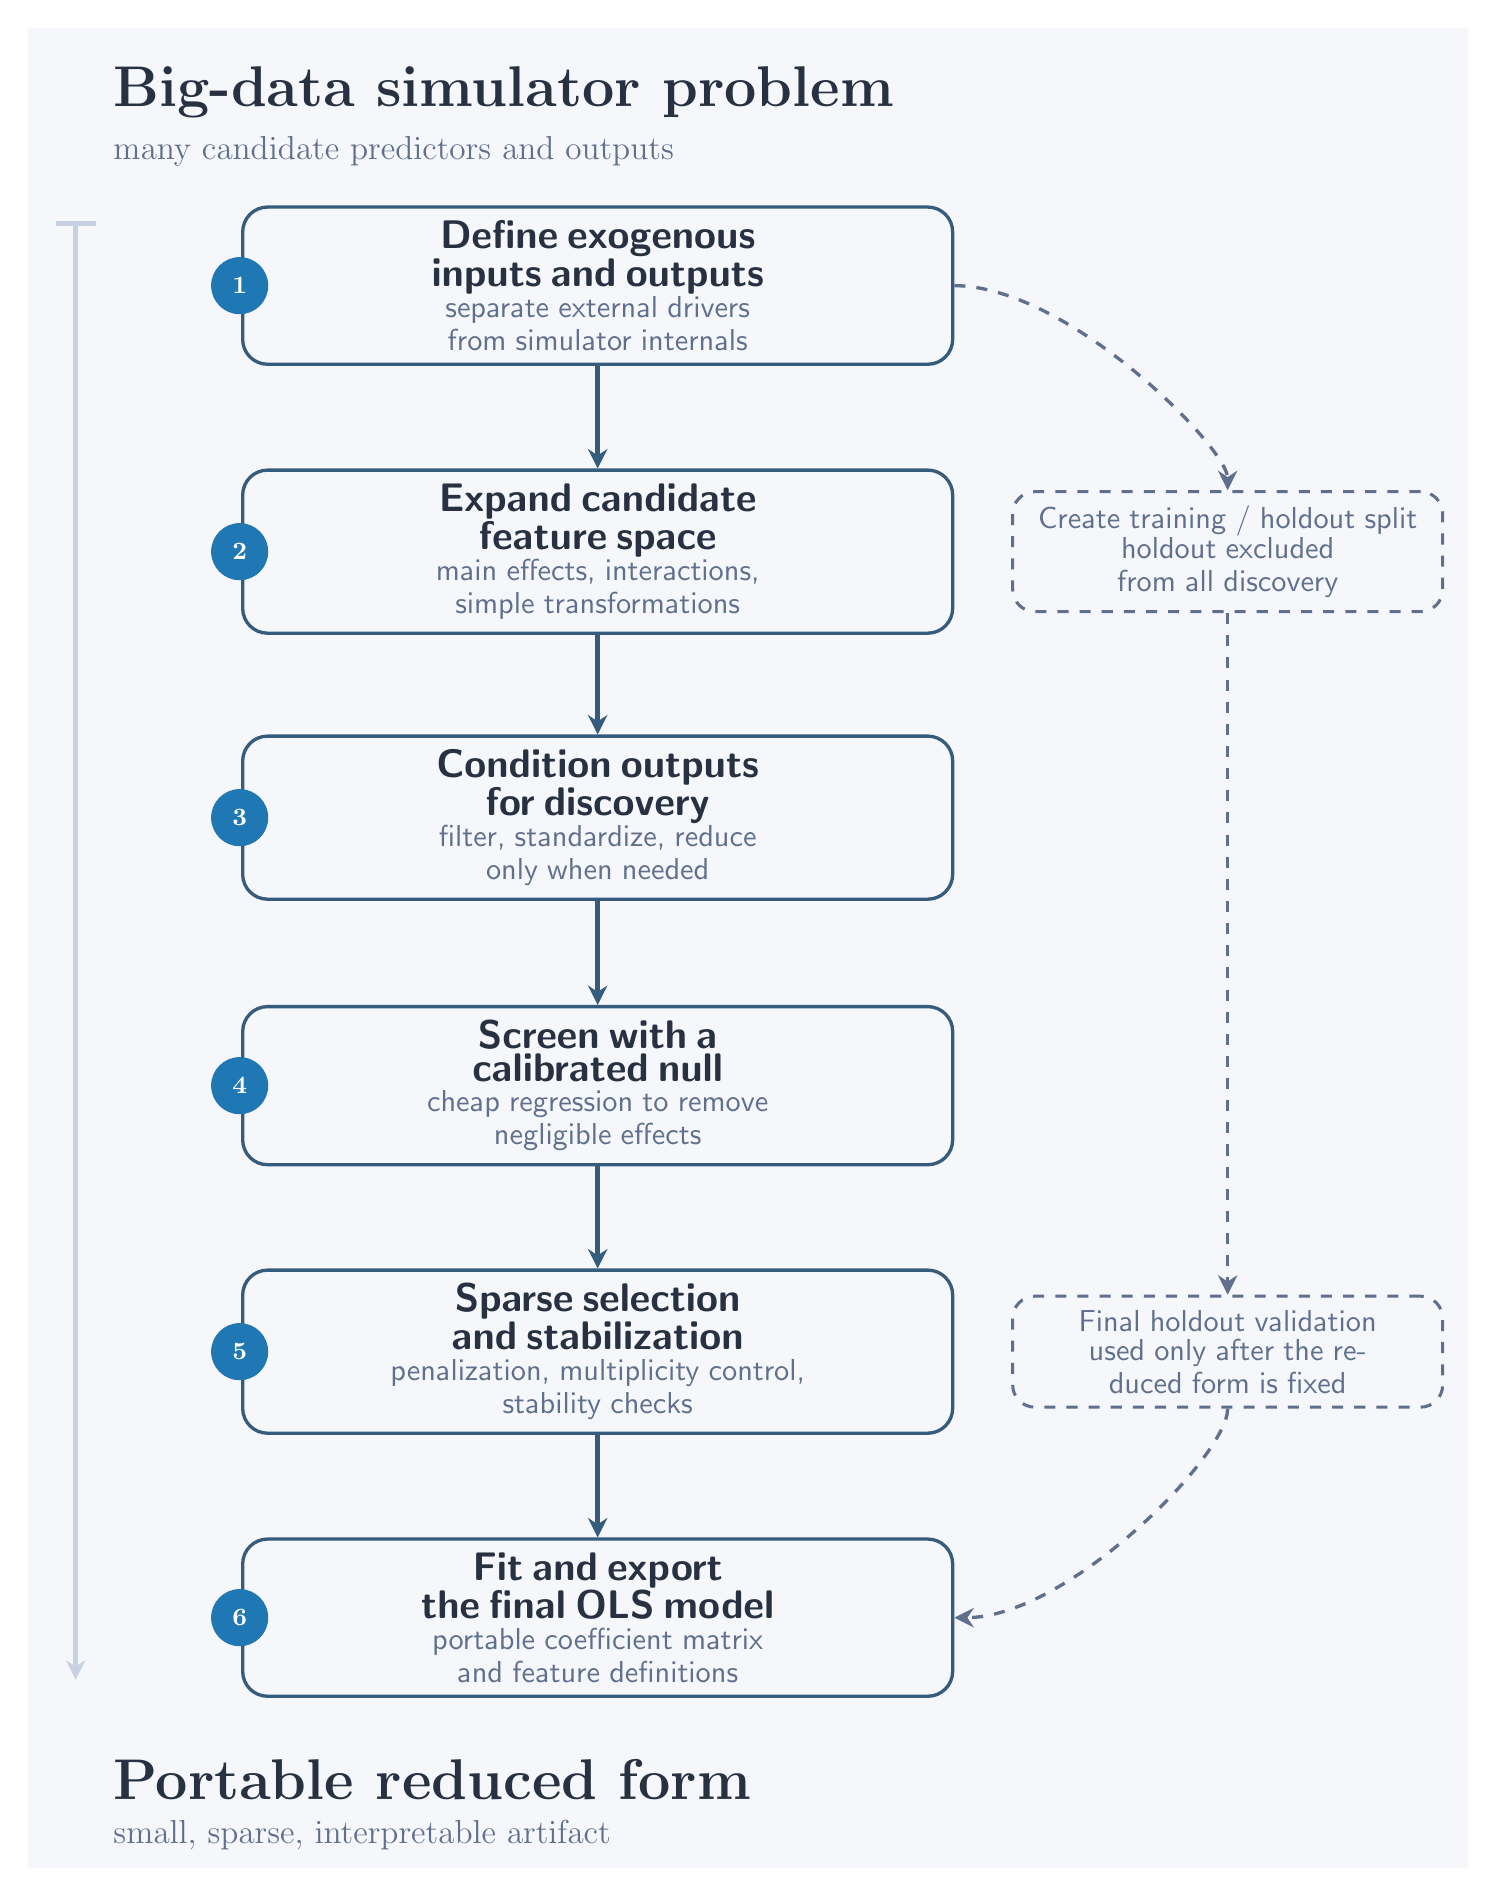
\begin{tikzpicture}[x=1in,y=1in,>=Stealth,font=\sffamily]

% canvas
\fill[figbg] (0,0) rectangle (7.20,9.20);

% header
\node[anchor=west,text=figdark,font=\bfseries\fontsize{20}{22}\selectfont]
  at (0.38,8.88) {Big-data simulator problem};
\node[anchor=west,text=figmid,font=\fontsize{12}{14}\selectfont]
  at (0.38,8.58) {many candidate predictors and outputs};

% footer
\node[anchor=west,text=figdark,font=\bfseries\fontsize{20}{22}\selectfont]
  at (0.38,0.44) {Portable reduced form};
\node[anchor=west,text=figmid,font=\fontsize{12}{14}\selectfont]
  at (0.38,0.16) {small, sparse, interpretable artifact};

% left guide — top flush with b1.north (8.22), bottom flush with b6.south (0.94)
\draw[figlight,line width=1.8pt] (0.24,8.22) -- (0.24,1.10);
\draw[figlight,line width=1.8pt] (0.14,8.22) -- (0.34,8.22);
\draw[figlight,line width=1.8pt,-{Stealth[length=7pt,width=7pt]}]
  (0.24,1.10) -- (0.24,0.94);

\tikzset{
  stage/.style={
    draw=figedge,
    fill=figbg,
    rounded corners=9pt,
    line width=1.2pt,
    minimum width=3.55in,
    minimum height=0.62in,
    text width=3.05in,
    align=center,
    inner sep=5pt
  },
  hold/.style={
    draw=figmid,
    fill=figbg,
    rounded corners=8pt,
    dash pattern=on 4pt off 4pt,
    line width=1.1pt,
    minimum width=2.15in,
    minimum height=0.52in,
    text width=1.95in,
    align=center,
    inner sep=5pt
  },
  badge/.style={
    circle,
    draw=figblue,
    fill=figblue,
    minimum size=0.28in,
    inner sep=0pt,
    text=white,
    font=\bfseries\small
  },
  mainflow/.style={
    draw=figedge,
    line width=1.6pt,
    -{Stealth[length=7pt,width=7pt]}
  },
  holdflow/.style={
    draw=figmid,
    dash pattern=on 4pt off 4pt,
    line width=1.2pt,
    -{Stealth[length=7pt,width=7pt]}
  }
}

% main boxes — 6 steps, x=2.85, step=1.332 from cy=7.91 to cy=1.25
% equal 0.28in white space above b1.top (8.22) and below b6.bot (0.94)
\node[stage] (b1) at (2.85,7.91)
  {\textcolor{figdark}{\bfseries\fontsize{14}{15}\selectfont Define exogenous\\inputs and outputs}\\[-1pt]
   \textcolor{figmid}{\fontsize{11}{12}\selectfont separate external drivers\\from simulator internals}};

\node[stage] (b2) at (2.85,6.58)
  {\textcolor{figdark}{\bfseries\fontsize{14}{15}\selectfont Expand candidate\\feature space}\\[-1pt]
   \textcolor{figmid}{\fontsize{11}{12}\selectfont main effects, interactions,\\simple transformations}};

\node[stage] (b3) at (2.85,5.25)
  {\textcolor{figdark}{\bfseries\fontsize{14}{15}\selectfont Condition outputs\\for discovery}\\[-1pt]
   \textcolor{figmid}{\fontsize{11}{12}\selectfont filter, standardize, reduce\\only when needed}};

\node[stage] (b4) at (2.85,3.91)
  {\textcolor{figdark}{\bfseries\fontsize{14}{15}\selectfont Screen with a\\calibrated null}\\[-1pt]
   \textcolor{figmid}{\fontsize{11}{12}\selectfont cheap regression to remove\\negligible effects}};

\node[stage] (b5) at (2.85,2.58)
  {\textcolor{figdark}{\bfseries\fontsize{14}{15}\selectfont Sparse selection\\and stabilization}\\[-1pt]
   \textcolor{figmid}{\fontsize{11}{12}\selectfont penalization, multiplicity control,\\stability checks}};

\node[stage] (b6) at (2.85,1.25)
  {\textcolor{figdark}{\bfseries\fontsize{14}{15}\selectfont Fit and export\\the final OLS model}\\[-1pt]
   \textcolor{figmid}{\fontsize{11}{12}\selectfont portable coefficient matrix\\and feature definitions}};

% number badges
\foreach \n/\y in {1/7.91,2/6.58,3/5.25,4/3.91,5/2.58,6/1.25}{
  \node[badge] at (1.06,\y) {\n};
}

% main arrows
\draw[mainflow] (b1.south) -- (b2.north);
\draw[mainflow] (b2.south) -- (b3.north);
\draw[mainflow] (b3.south) -- (b4.north);
\draw[mainflow] (b4.south) -- (b5.north);
\draw[mainflow] (b5.south) -- (b6.north);

% holdout lane — h1 aligned with b2 (6.58), h2 aligned with b5 (2.58)
\node[hold] (h1) at (6.00,6.58)
  {\textcolor{figmid}{\fontsize{10.5}{11.5}\selectfont Create training / holdout split}\\[-1pt]
   \textcolor{figmid}{\fontsize{10.5}{11.5}\selectfont holdout excluded from all discovery}};

\node[hold] (h2) at (6.00,2.58)
  {\textcolor{figmid}{\fontsize{10.5}{11.5}\selectfont Final holdout validation}\\[-1pt]
   \textcolor{figmid}{\fontsize{10.5}{11.5}\selectfont used only after the re-\\duced form is fixed}};

% holdout connectors
\draw[holdflow]
  (b1.east)
  .. controls (5.20,7.91) and (6.00,7.10) ..
  (h1.north);

\draw[holdflow]
  (h1.south) -- (h2.north);

\draw[holdflow]
  (h2.south)
  .. controls (6.00,2.06) and (5.20,1.25) ..
  (b6.east);

\end{tikzpicture}%
}
\caption{Reproducible workflow for constructing an interpretable reduced-form surrogate from a large simulator. The main vertical pipeline defines the external problem, expands a candidate feature space, conditions the output space, screens features against a calibrated null, performs sparse reduction, and ends in an exportable ordinary least squares reduced form. A separate holdout lane is reserved before any screening or selection step and is used only for final validation.}
\label{fig:workflow-generic-vertical}
\end{figure}

\section{Workflow}
\label{sec:workflow}

Figure~\ref{fig:workflow-generic-vertical} summarizes the workflow as a six-stage reduction pipeline with a separate holdout lane. The holdout split is created immediately after the external interface is defined and is not touched again until final validation.

\subsection{Define exogenous inputs and outputs}

The workflow begins by defining the external interface to be approximated. The analyst must identify the exogenous drivers that will be varied outside the simulator and the outputs that matter for downstream use. The goal may not be to reproduce every simulator state, but to define a portable map from external drivers to reported outputs. At this stage we also create a training--holdout split. A holdout fraction $\eta_{\mathrm{hold}}$ in the range of roughly 5\%--20\% is a practical starting point, with 10\% often reasonable when the overall run count is large enough to support both discovery and validation. The holdout sample is excluded from every adaptive stage that follows.

\subsection{Expand candidate feature space}

The next step expands the external inputs into an algebraic candidate library. A practical starting library contains all first-order terms, scientifically plausible pairwise products, and a restricted set of simple nonlinear transformations. The library should be broad enough to capture interaction and curvature effects, but still constrained so that every retained term can later be written down and interpreted directly. This is the stage at which the workflow commits to algebraic portability: even when later discovery diagnostics are used, candidate terms are restricted to forms that can appear in the final exported surrogate.

\subsection{Condition outputs for discovery}

The response side is conditioned in parallel. Let $Y_m$ denote scalar output $m$ across runs. Outputs with variance below a problem-specific floor $\varepsilon_{\mathrm{var}}$ are removed as structural zeros or near-deterministic quantities. We also filter outputs with negligible variation relative to scale using a simple signal-to-noise ratio,
\[
\mathrm{SNR}_m = \frac{\mathrm{Var}(Y_m)}{\mathbb{E}[Y_m^2] + \delta},
\]
where $\delta > 0$ is a small numerical-stability constant. A practical starting rule is to remove outputs with $\mathrm{SNR}_m < \varepsilon_{\mathrm{snr}}$, with $\varepsilon_{\mathrm{snr}} \approx 10^{-2}$ often serving as a useful default because it filters outputs whose variation is negligible relative to their overall energy. When the number of scalar outputs is too large for direct discovery, the standardized response matrix can be reduced temporarily to $r$ components capturing a target fraction $\tau_{\mathrm{PCA}}$ of retained variance; values near $\tau_{\mathrm{PCA}}=0.9$ are a common starting point. The reduced scores are used only for intermediate discovery and screening, not for the final exported model.  % TODO: PCA is only example of a dimension reduction method. It _happens_ to be the one we chose for the BSM case study, but even in the problem set up section we note it could be any reduction technique or basis approximation. Rewrite the second to last sentence to be more general or to make explicity that a target PCA variance is just one method. And what do you mean by "reduced scores"? The reduced output space? Is "scores" a common term in this space?

\subsection{Screen with a calibrated null}

The first major reduction step is a deliberately liberal multivariate regression screen. Let $X^{(0)}$ denote the expanded candidate matrix after scaling and let $Y^{(f)}$ denote the filtered scalar-output matrix. For each candidate feature $j$, we fit ordinary least squares across all columns of $Y^{(f)}$ and summarize its overall effect size by
\[
T_j^{\mathrm{obs}} = \lVert \widehat{\beta}_{j\cdot}^{\,\mathrm{obs}} \rVert_2,
\]
where $\widehat{\beta}_{j\cdot}^{\,\mathrm{obs}}$ is the row of estimated coefficients associated with feature $j$.

Large coefficients can arise by chance in high-dimensional problems, so the screen is calibrated against an empirical null rather than against asymptotic theory alone. We permute the rows of $Y^{(f)}$ relative to $X^{(0)}$ for $B$ replicates, recompute the same statistic,
\[
T_j^{(b)} = \lVert \widehat{\beta}_{j\cdot}^{\,(b)} \rVert_2,
\qquad b=1,\dots,B,
\]
and estimate permutation $p$-values by the usual Monte Carlo tail fraction. Multiple testing is then controlled with the Benjamini--Hochberg false discovery rate procedure \citep{BenjaminiHochberg1995}. Because this is a screening stage rather than a final inferential statement, a relatively permissive target such as $q_{\mathrm{screen}} \approx 0.10$ is often appropriate: it removes clearly negligible effects while reducing the risk of early false exclusions.

\subsection{Sparse selection and stabilization}

The screened set is then enriched and stabilized before final estimation. Interaction candidates can be prioritized by fitting tree-based models to the reduced responses and computing SHAP interaction values \citep{LundbergLee2017}. A practical rule is to aggregate interaction strength across retained response components and retain only pairs exceeding a high permutation-null quantile $c_{\mathrm{int}}$, for example a 99th or 99.5th percentile threshold, so that only exceptional interactions are carried forward. Nonlinear main effects can be flagged with generalized additive model diagnostics \citep{HastieTibshirani1990}; when curvature is detected, the smooth term is approximated with the best-fitting member of a restricted parametric library such as quadratic, logarithmic, inverse, or exponential transforms so that the final representation remains algebraic.

The screened and enriched terms are then combined into an updated predictor matrix $X^{(1)}$. Sparse selection is carried out on the reduced response representation rather than directly on all scalar outputs. For each retained reduced-response score, we fit an $\ell_1$-penalized linear model \citep{Tibshirani1996}, choosing the penalty level with the extended Bayesian information criterion \citep{ChenChen2008}. A value near $\gamma_{\mathrm{EBIC}} = 0.5$ is a reasonable default when the candidate space is large, because it penalizes model size more strongly than ordinary BIC while remaining less conservative than extreme sparsity rules. Because selected supports can change with sample size and resampling variation, we recommend explicit stability targets before accepting the final support; for example, Jaccard overlap above 0.75 for selected supports and Spearman correlation % TODO: does Jaccard overlap and Spearman correlation have a canonical citation?
above 0.9 for coefficient magnitudes provide a practical starting standard for stable recovery. A final inferential filter can then remove terms whose interval estimates still include zero.

\subsection{Fit and export the final OLS model}

Once the support set $S$ is fixed, the workflow returns from the reduced response representation to the original scalar outputs. The final reduced form is estimated by unpenalized multivariate ordinary least squares on $Y$ using only the selected columns $X_S$. This refit removes shrinkage from the support-recovery stage and yields a direct coefficient matrix on the original outputs. Ordinary least squares is used here deliberately: not because the simulator is assumed to be globally linear in the raw inputs, but because the selected algebraic feature map makes a transparent and portable final representation possible.

Final validation is performed only once, on the holdout sample reserved at the beginning of the workflow. When sample size permits, a holdout fraction near 10\% is often a useful compromise between preserving training information and retaining a meaningful external check. Predictive performance can be summarized with normalized root mean squared error or related scale-adjusted metrics, while interpretation is tied to the retained algebraic terms themselves rather than to latent variables or local explanation maps. The exported artifact consists of the input and output definitions, preprocessing rules, selected feature definitions, coefficient matrix, and supporting metadata needed to evaluate the reduced form outside the original simulator environment.

\section{Case Study: Bioenergy Scenario Model}
\label{sec:case}

The Bioenergy Scenario Model (BSM) provides the motivating application for the workflow and is used here as a demanding statistical test case. The BSM is a large system dynamics model developed at the National Renewable Energy Laboratory to study U.S. biofuels deployment over multiple decades \citep{PetersonEtAl2013}. Its scientific value comes from representing interacting technology, infrastructure, market, and policy processes in a single simulation environment. Those same features make it a useful case for reduced-form construction: the simulator is rich enough to generate many coupled outputs, yet complex enough that repeated direct use can be cumbersome in downstream studies.

For the present study, we impose explicit input and output boundaries before any statistical modeling begins. The input side is restricted to 160 exogenous drivers that can be sampled and communicated outside the full simulator, consisting of 158 scalar inputs and 2 boolean variables. The output side is restricted to 635 time-series quantities selected for downstream relevance, each recorded annually from 2015 through 2051, yielding 23{,}495 scalar responses after flattening. The objective is not to emulate every internal state of BSM, but to construct a portable reduced form for a clearly defined external interface between exogenous drivers and reported outputs.

Simulation runs are generated from a Latin hypercube design over the exogenous inputs \citep{McKayEtAl1979}. This design provides broad coverage of the sampled domain while remaining straightforward to reproduce. A fixed 10\% holdout set is removed before screening, discovery, selection, or final estimation so that all reported predictive metrics remain genuinely out of sample. The resulting dataset is large enough to support the staged workflow, but still far smaller than what would typically be required for direct output-by-output global sensitivity analysis over the same response set. % TODO: this last sentence is a little out of context. Either reframe the 'big data problem' as more broad than sensitivity analysis or make it more explicit in the introduction that sensitivity analysis drove the need for performant statistical methods.

BSM is a demanding test case for three reasons. First, the response is high-dimensional: even after restricting attention to selected outputs, the problem still contains 23{,}495 scalar responses. Second, feature expansion rapidly creates a large candidate predictor space once interactions and simple nonlinear transformations are introduced. Third, the end product must be usable outside the original simulator environment, which places a premium on transparent algebraic structure rather than on a surrogate that can only be queried through a specialized software stack. The case study therefore evaluates whether the workflow can convert a large, coupled simulator dataset into a smaller statistical artifact that remains accurate, interpretable, and portable.

\section{Results}
\label{sec:results}

The results are reported with the workflow's objectives in mind: substantial dimensionality reduction, strong out-of-sample predictive fidelity, interpretable retained structure, and a final artifact that can be evaluated without rerunning the full simulator. Table~\ref{tab:results-summary} collects the main verified stagewise counts and holdout metrics used throughout this section.

\subsection{Reduction of predictor and output complexity}

The workflow materially reduced both sides of the statistical problem. On the predictor side, the 160 exogenous inputs were expanded to an algebraic candidate library of approximately 26{,}560 terms. %TODO: expand this sentence to explain where the 26,560 terms came from (i.e., interactions. Make sure the math adds up
On the output side, the modeling target remained the full set of 23{,}495 scalar responses, but intermediate discovery stages were carried out on a reduced response representation to keep computation tractable. After output filtering and standardization, the first 39 principal components captured 90\% of the retained output variance and provided the working response representation for interaction and nonlinearity discovery.

Empirical-null regression screening then reduced the working predictor set to 349 terms using Benjamini--Hochberg control at $q=0.10$. Auxiliary discovery stages identified 367 statistically exceptional interaction pairs by retaining only pairs above the 99.5th percentile of the permutation null, and identified 112 nonlinear transformations by carrying forward only those effects for which a generalized additive model indicated curvature and a simple parametric replacement fit well. After sparse reduction and stabilization, the final support contained 340 retained predictors derived from 62 first-order inputs. The main result of this stage is therefore not a marginal trimming of a large model, but a transition from a broad candidate construction to a portable algebraic support small enough to estimate, inspect, and export.

\subsection{Predictive fidelity on unseen simulator runs}

Predictive performance was assessed only on the fixed 10\% holdout sample reserved before screening, discovery, selection, and estimation. The intermediate penalized model achieved holdout nRMSE 0.0859 %TODO: need to define how we normalized RMSE here and define nRMSE if it's the first time we used the acronym
. After transferring the selected support to an unpenalized ordinary least squares refit, the final reduced form achieved holdout nRMSE 0.0445. The improvement is practically important because it shows that sparsity-inducing selection and final unbiased estimation served different purposes in the workflow: penalization recovered a compact support, while the final OLS refit improved prediction by reducing shrinkage in the retained coefficients, consistent with the rationale behind post-selection refitting and relaxed lasso procedures \citep{Tibshirani1996,Meinshausen2007}.

Representative held-out predicted-versus-observed comparisons for selected outputs are shown in Figure~\ref{fig:results-scatter}. The points cluster tightly around the 45$^\circ$ line across both production and price outputs, which is consistent with the low aggregate holdout error. Figure~\ref{fig:results-timeseries} complements this view by showing that the reduced form also reproduces representative temporal trajectories rather than only pointwise output summaries.

\begin{figure}[t]
\centering
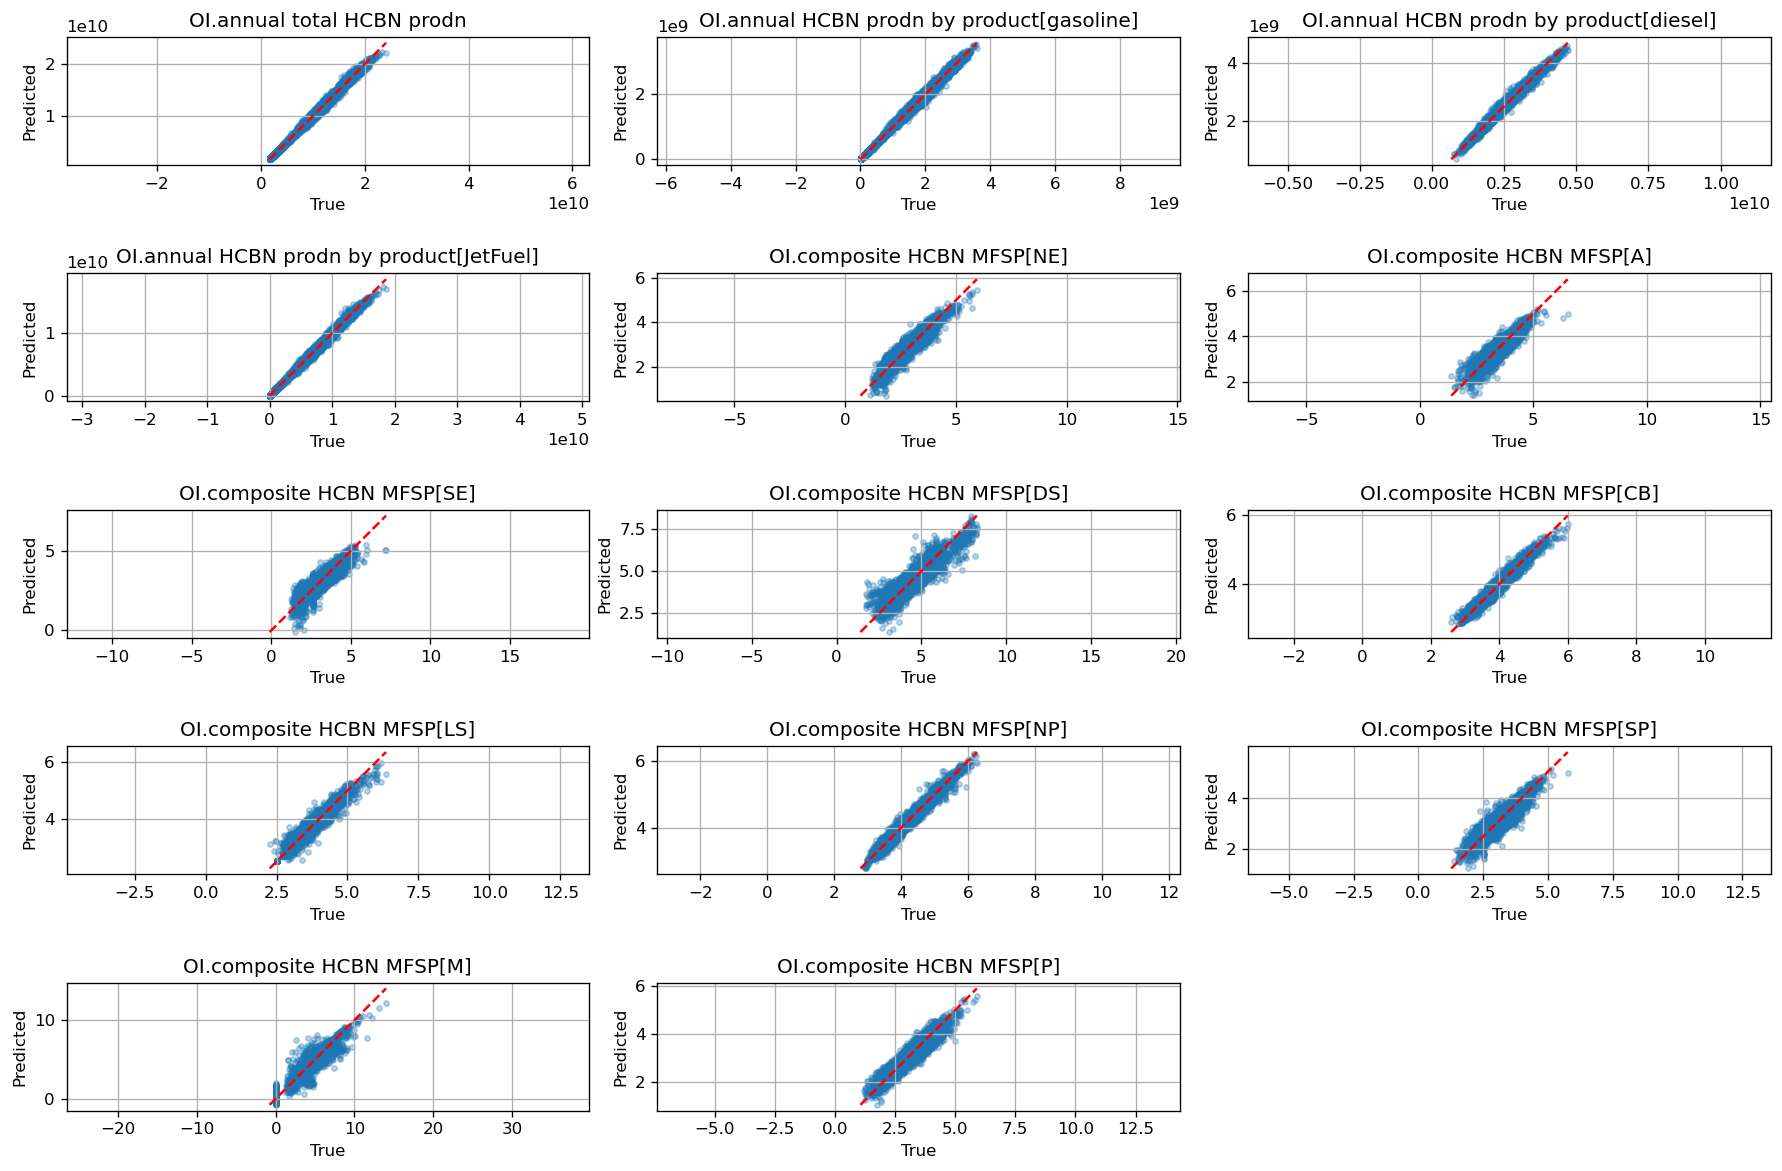
\includegraphics[width=\linewidth]{results_scatter_selected_outputs.png}
\caption{Predicted versus observed values for representative held-out BSM outputs under the final OLS reduced form. The selected panels show close agreement with the full simulator across production and price outputs and complement the aggregate holdout nRMSE summary.}
\label{fig:results-scatter}
\end{figure}

\begin{figure}[t]
\centering
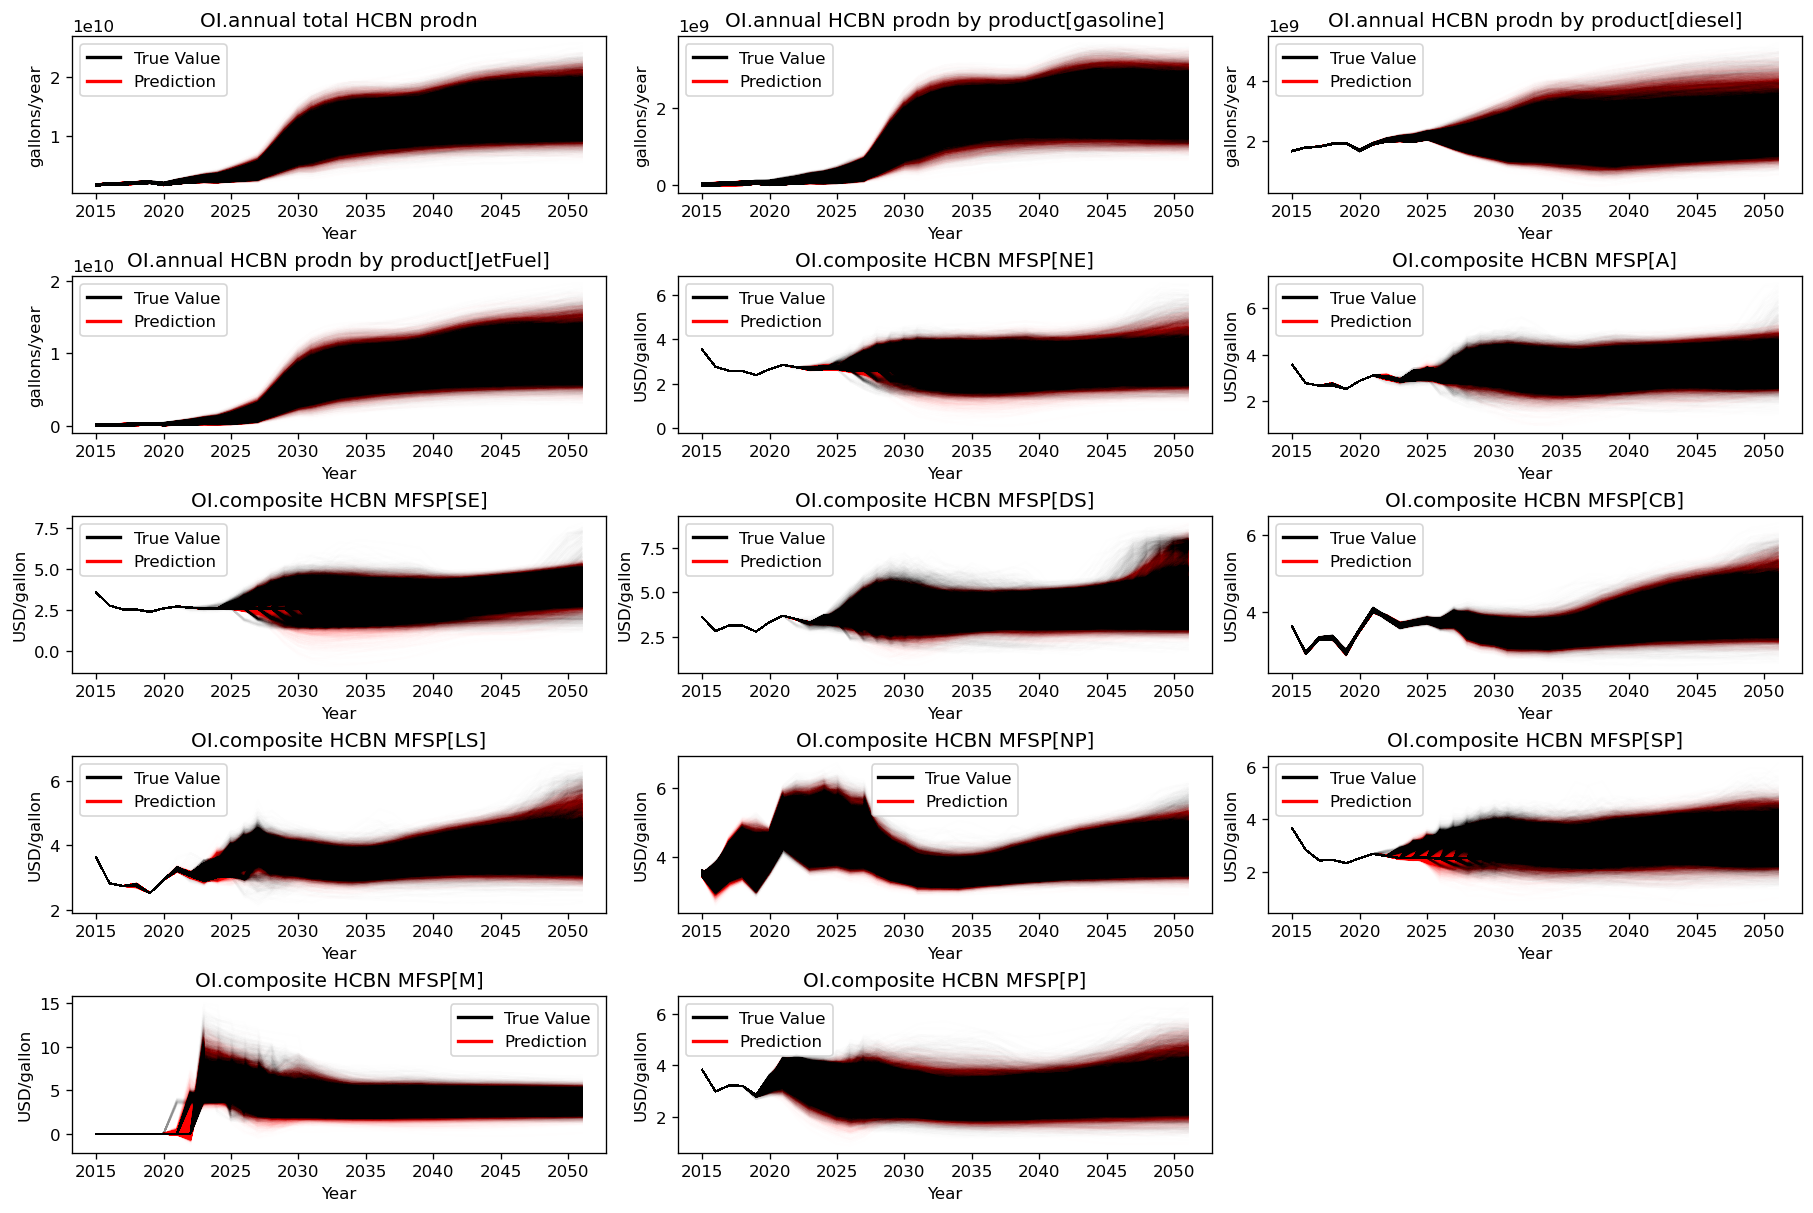
\includegraphics[width=\linewidth]{results_timeseries_selected_outputs.png}
\caption{Representative held-out time-series comparisons between the final reduced form and the full BSM. Across selected outputs, the reduced form tracks both level and trajectory shape over time.}
\label{fig:results-timeseries}
\end{figure}

\subsection{Structure of retained effects}

The final reduced form is not merely a sparse additive fit on raw inputs. Interaction terms dominate the retained support, and the selected model also includes 37 nonlinear transformations. More than half of the retained interactions span multiple pathways rather than remaining within a single local module. Statistically, this matters because it shows that the workflow is discovering coupled structure that would be invisible to a main-effects-only reduction.

The retained support nevertheless remains interpretable in the sense required by the paper's design objective. Every selected term is either a first-order input, an explicit pairwise product, or a simple named transformation. Figure~\ref{fig:results-feature-composition} summarizes that composition, and Figure~\ref{fig:results-interaction-density} shows that many retained interactions connect different BSM modules rather than remaining within a single local block. Interpretation therefore occurs directly on the algebraic support rather than through post hoc explanations of a black-box predictor. For this application, interpretability does not mean that every coefficient has a simple domain meaning in isolation; it means that the final surrogate is expressed in a finite, inspectable set of terms that can be audited, communicated, and reused.

\begin{figure}[t]
\centering
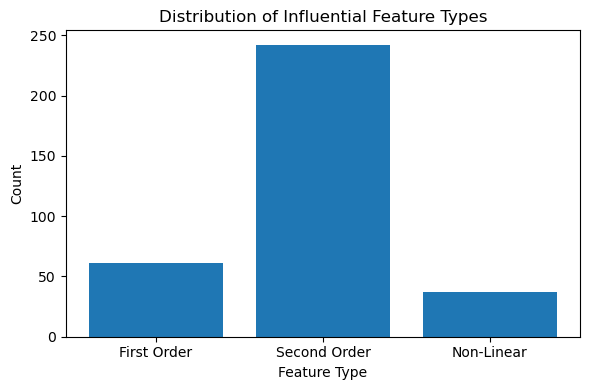
\includegraphics[width=0.72\linewidth]{results_feature_type_composition.png}
\caption{Composition of the retained predictor support by term type in the final reduced form. Interaction terms dominate the retained support, with first-order and nonlinear terms still present in nontrivial numbers.}
\label{fig:results-feature-composition}
\end{figure}

\begin{figure}[t]
\centering
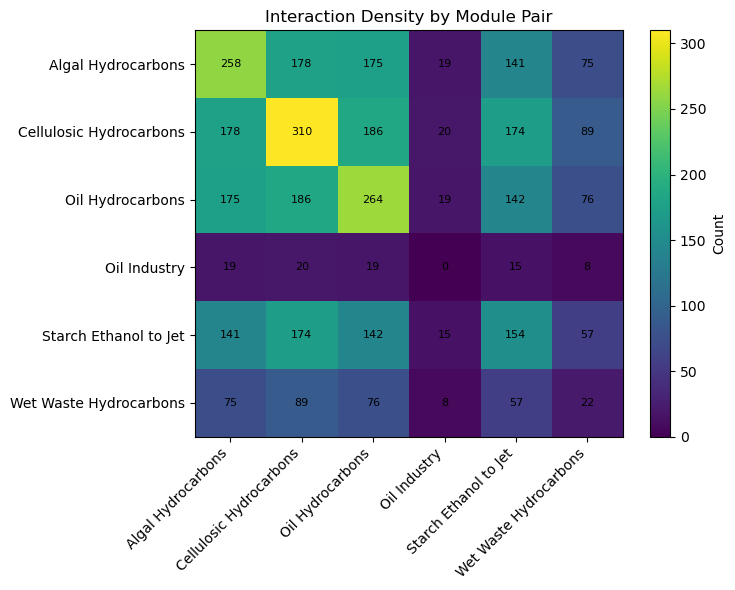
\includegraphics[width=0.82\linewidth]{results_interaction_density_heatmap.png}
\caption{Density of retained interaction pairs by BSM module pair. The interaction structure is not confined to within-module terms; substantial cross-module coupling remains in the final reduced form.}
\label{fig:results-interaction-density}
\end{figure}

\subsection{Practical value of the final reduced form}

The main practical result is the form of the exported artifact itself. The workflow ends with an ordinary least squares coefficient matrix on 340 retained predictors rather than with a software-bound emulator object. Combined with the feature definitions and preprocessing rules, this gives a reduced form that can be evaluated outside the original BSM environment and incorporated into downstream studies that need a transparent approximation rather than repeated simulator execution.

This practical gain is distinct from raw predictive accuracy. A black-box surrogate might also predict well, but the objective here is a portable reduced form that can support later sensitivity, scenario, and integration analyses without re-implementing the full simulator stack. In that sense, the results show that the workflow did not merely fit a smaller model; it converted a large simulator problem into an interpretable statistical artifact that is substantially easier to inspect and reuse.

\begin{table}[t]
\centering
\caption{Verified stagewise reduction and performance summary for the BSM reduced form. Discovery-stage counts are reported separately from the final retained support because they serve different roles in the workflow.}
\label{tab:results-summary}
\begin{tabular}{lll}
\hline
Quantity & Value & Role in workflow \\
\hline
Exogenous inputs & 160 & external driver set \\
Expanded candidate library & $26{,}560$ & initial algebraic predictor space \\
Scalar responses & 23{,}495 & final multivariate prediction target \\
Retained principal components & 39 & 90\% of retained output variance \\
Empirical-null screen retained terms & 349 & working predictor set after screening \\
Exceptional interaction pairs identified & 367 & discovery-stage interaction candidates \\
Nonlinear transformations identified & 112 & discovery-stage nonlinear candidates \\
Intermediate penalized-model holdout nRMSE & 0.0859 & support recovery stage \\
Final retained predictors & 340 & exported algebraic support \\
Unique first-order inputs represented & 62 & direct drivers in final support \\
Final OLS holdout nRMSE & 0.0445 & final predictive fidelity \\
\hline
\end{tabular}
\end{table}

\FloatBarrier

\section{Discussion}
\label{sec:discussion}

We present a statistical workflow for reducing a large simulator problem to an interpretable reduced form. In the BSM case study, that workflow converted a simulator interface with 160 exogenous inputs and 23{,}495 scalar responses into a portable ordinary least squares artifact with 340 retained predictors derived from 62 first-order inputs. The substantive importance of this result lies in the combination of properties rather than in any one metric alone: the final model remains accurate on held-out simulator runs, is expressed in explicit algebraic terms, and can be evaluated without rerunning the full simulator.

This workflow perspective matters because the underlying statistical problem is heterogeneous. Interface definition, calibrated screening, structured discovery, sparse selection, final estimation, and validation solve different problems and therefore should not be collapsed into a single modeling step. The empirical-null screen is intentionally permissive because its purpose is to remove negligible effects while protecting against early false exclusions. The reduced-response discovery stages are computational devices for exposing structure that would be difficult to detect directly across a very large collection of scalar outputs. The final ordinary least squares refit serves yet another purpose by removing shrinkage bias and producing the transparent coefficient matrix required for export. Treating these stages as distinct is central to the paper's design and helps explain why the workflow ends in an interpretable algebraic object rather than in the intermediate models used during discovery. A highly flexible emulator could in principle offer strong predictive accuracy, but it would not automatically deliver the compact symbolic representation needed for downstream auditing, integration, or communication.

The results should nevertheless be interpreted with appropriate caution. First, the final surrogate remains linear in the selected feature library, so higher-order nonlinearities and discontinuous regime changes can still be missed; nonlinear systems can have substantial interaction contributions that are not well represented by lower-order approximations alone \citep{HommaSaltelli1996} % TODO: no, Homma and Saltelli is not the right citation for this. They cite another paper in their work that says higher order interactions can be important. Find that citation and use it here, don't cite Homma and Saltelli 1996 here
. Second, the screening and discovery stages can be computationally demanding, particularly the empirical-null calibration step. Third, the reduced form is validated on held-out runs drawn from the same overall experimental design, so the reported accuracy should be interpreted as within-design generalization rather than unrestricted extrapolative validity.

Within those limits, the BSM example shows that large simulator problems can be reduced systematically rather than heuristically. The broader implication is that interpretable reduced forms need not be limited to small models or hand-selected predictors. When the workflow is staged carefully, high-dimensional simulator studies can be transformed into auditable statistical artifacts that support later prediction, sensitivity analysis, scenario exploration, and model integration without requiring repeated direct simulator execution.

\section{Conclusion}
\label{sec:conclusion}

The main contribution of this paper is a workflow template for interpretable reduced-form modeling in large-simulator settings. Rather than treating screening, discovery, selection, estimation, and validation as interchangeable modeling choices, the paper organizes them as separate statistical tasks with different objectives and then reconnects them in a single exportable pipeline. % TODO: rephrase this to not use phrases like "the main contribution of this paper" and "the paper"

The case study shows that this design can produce a compact surrogate that remains both accurate and algebraically transparent. More broadly, the paper argues that interpretable statistical compression should be treated as a first-class data-science task for large simulators whenever downstream use requires an artifact that can be audited, communicated, and embedded in other analyses without repeated direct simulator execution.

\section{Reproducibility and Released Artifacts}
\label{sec:reproducibility}

Reproducibility in this paper is defined at the workflow-and-artifact level. The goal is to make the reduced-form construction auditable and reusable from the documented external interface, not to require repeated execution of simulator internals that may not be portable outside the original modeling environment.

Upon clearance, the intended release package is a project repository containing the pipeline code together with the reduced-form artifact bundle: feature definitions, input and output metadata, the coefficient matrix, and supporting summary quantities needed to evaluate the surrogate. The Supplementary Material will document these components and provide the metadata needed to connect the released artifact to the workflow described in the paper. % TODO: don't say things like "upon clearance" but write this section as though the workflow artifacts and code are already released

% refer to section numbers by their labels in the paper
%\section{}\label{}

%% Table %%
%%%%%%%%%%%%%%%%%%%%%%
%\begin{table}
%\caption{}\label{}
%\end{table}

%% Figure %%
%%%%%%%%%%%%%%%%%%%%%%
%\begin{figure}[t]
%\includegraphics{}
%\caption{}\label{}
%\end{figure}

%% Theorem %%
%%%%%%%%%%%%%%%%%%%%%%
%%\begin{thm}[]\label{} Theorem
%%\end{thm}

%% Proof %%
%%%%%%%%%%%%%%%%%%%%%%
%\begin{proof}
%\end{proof}


%% Supplementary Material is required for reproducibility check
%% List its contents and links to public repositories
%% Provide description of Supplementary Material in \esmdescription{}
%%%%%%%%%%%%%%%%%%%%%%
\begin{esm}
\esmtitle{Supplementary Material}
\esmdescription{} % TODO: fill out this section assuming a github repo exists with all the artifacts readily available for reproduction
\esmfilename{}
\end{esm}

%% Appendices %%
%%%%%%%%%%%%%%%%%%%%%%
\begin{appendix}
\section{Appendix section}
\end{appendix}

%% Acknowledgements %%
%%%%%%%%%%%%%%%%%%%%%%
\begin{acknowledgement}%[title={Acknowledgments}]
% TODO: fill out this section with acknowledgements of National Laboratory of the Rockies collaborators and internal reviewers that made the workflow and manuscript better
\end{acknowledgement}

%% Funding %%
%%%%%%%%%%%%%%%%%%%%%%
\begin{funding}
% TODO: fill out this section by saying funding was provided by the Bioenergy Technologies Office of the Department of Energy
\end{funding}

\bibliographystyle{jds}
\bibliography{ref_v3}

\end{document}
